% Volume III chapter: Mellin zeros of generalised gamma convolutions and the pairing of the zeros of beta and zeta. Sources: misc/reviews/nick-mellin/mellin/mellin_chapter.tex lines 1 to 197 and misc/reviews/nick-pairing/pairing/pairing_chapter.tex lines 1 to 190; referees misc/research/directions/opus/vol3/MELLIN.md (MM1 to MM4) and PAIR.md (M1 to M6); numbers misc/vol3/verify/PAIR/results.md. 17 Nov 2026.
% Figures kept: fig/v3/fig_mellin_velocity.pdf, fig/v3/fig_pairing.pdf. The figure of the five tracked zeros (fig_mellin_tracks) is dropped: its coarse 25 step run misplaces zero 4 at lambda=0.6 (0.472 against 0.507), so it must be redrawn with the adaptive steps before it can be used.
\label{ml:ch:mellin}

Chapter~\ref{kr:ch:route} ends with a question, Problem~\ref{kr:prob:mellin}: is there a condition on the Thorin measure of an exponential series under which the zeros of its Mellin transform lie on one line? The Kolmogorov law is the case $\{2n^2\}$, and RH says that it satisfies such a condition. This chapter embeds that law in a one parameter family of exponential series whose Thorin measures differ only by a shift of the lattice, follows the zeros of the Mellin transform through the family, and records what the computation shows. At one end of the family the Mellin transform is Dirichlet's beta function, at the other it is $\eta(w-1)=(1-2^{2-w})\zeta(w-1)$. The zeros move continuously from the zeros of $\beta$ to the zeros of $\zeta$ and of a Dirichlet polynomial, and in between they lie on no common line. The family does not answer Problem~\ref{kr:prob:mellin}. It shows that a condition invariant under the shift of the lattice is not enough. Nothing here bears on RH. The chapter is from an unrefereed note of Polson (November 2026), with the Vol I function $Z_t$ and its theorem (Theorem~\ref{lv:thm:meixner}) cited instead of reproved. Floating point results are marked computed; the rest is proved unless a remark says heuristic.

\section{Mellin transforms of exponential series and the family $X_\lambda$}\label{ml:sec:family}
Let $0<\lambda_1<\lambda_2<\cdots$ with $\sum1/\lambda_n<\infty$ and $X=\sum_nE_n/\lambda_n$, with independent unit exponentials $E_n$. Then $X$ is a GGC with Thorin measure $\sum_n\delta_{\lambda_n}$ and Laplace transform $L(u)=\prod_n(1+u/\lambda_n)^{-1}$. The partial fractions of $L$ give the coefficients $c_n=\prod_{m\ne n}(1-\lambda_n/\lambda_m)^{-1}$ and the density $\sum_nc_n\lambda_ne^{-\lambda_nx}$ (Section~\ref{kr:sec:problems} states the same series for the Kolmogorov law; the residue form is Proposition~\ref{fm:prop:residue}).
\begin{theorem}\label{ml:thm:mellin}
Suppose that $\sum_n|c_n|\lambda_n^{-\sigma}<\infty$ for some $\sigma>0$ and that $P(X>x)=\sum_nc_ne^{-\lambda_nx}$ for $x>0$. Then, for $\Re s\ge\sigma$,
\[
\mathbb E\,X^{s}=\Gamma(1+s)\,D(s),\qquad D(s)=\sum_nc_n\,\lambda_n^{-s},
\]
and for $\Re s>0$
\[
\begin{gathered}\Gamma(s)\,\mathbb E\,X^{-s}=\int_0^\infty u^{s-1}L(u)\,du,\\ \text{so that, with $D$ continued analytically,}\quad D(-s)=\frac{\sin\pi s}{\pi}\int_0^\infty u^{s-1}L(u)\,du .\end{gathered}
\]
\end{theorem}
\begin{proof}
The density is $\sum c_n\lambda_ne^{-\lambda_nx}$, integrated termwise by absolute convergence, and $\int_0^\infty x^s\lambda e^{-\lambda x}dx=\Gamma(1+s)\lambda^{-s}$. The second identity is $\Gamma(s)x^{-s}=\int_0^\infty u^{s-1}e^{-ux}du$ averaged over $X$, and the third uses $\Gamma(s)\Gamma(1-s)=\pi/\sin\pi s$.
\end{proof}
The Mellin transform of an exponential series is a Gamma function times a Dirichlet type series whose coefficients are the residues of the Laplace transform, and the zeros of interest are those of $D$. For the Kolmogorov law, $\lambda_n=2n^2$, $c_n=2(-1)^{n-1}$ and $D(s)=2^{1-s}\eta(2s)$. The reflection formula expresses $D(-s)$ as the Mellin transform of $L$, whose reciprocal lies in the Laguerre and P\'olya class with zeros at $-\lambda_n$.

For $\lambda>0$ let $X_\lambda=\sum_{k\ge0}\mathrm{Exp}(2(k+\lambda)^2)$, the sum of independent exponentials with these rates. We write $Z_{2\lambda}$ for the function $Z_t$ of Theorem~\ref{lv:thm:meixner} at $t=2\lambda$, so that
\[
Z_{2\lambda}(w)=\sum_{k\ge0}(-1)^k\frac{(2\lambda)_k}{k!}\,(k+\lambda)^{-w},\qquad \Gamma(w)Z_{2\lambda}(w)=\int_0^\infty t^{w-1}\big(2\cosh\tfrac t2\big)^{-2\lambda}dt,
\]
the series for $\Re w>2\lambda-1$ and the integral for $\Re w>0$. By Theorem~\ref{lv:thm:meixner}, $Z_{2\lambda}$ is entire, $Z_{1}(w)=2^w\beta(w)$ with $\beta(w)=\sum_{k\ge0}(-1)^k(2k+1)^{-w}$ the Dirichlet beta function, and $Z_{2}(w)=\eta(w-1)$. In terms of the parameter $\lambda$ of $X_\lambda$ these are the ends $\lambda=\frac12$ and $\lambda=1$.
\begin{theorem}\label{ml:thm:family}
For $\lambda>0$:
\begin{enumerate}
\item $\mathbb Ee^{-uX_\lambda}=|\Gamma(\lambda+i\sqrt{u/2})|^2/\Gamma(\lambda)^2$, and the Thorin measure of $X_\lambda$ is $\sum_{k\ge0}\delta_{2(k+\lambda)^2}$.
\item $c_k=\dfrac{2(-1)^k\,\Gamma(k+2\lambda)}{\Gamma(\lambda)^2\,k!\,(k+\lambda)}$.
\item With $w=2s+1$, $\ D_\lambda(s)=\dfrac{2^{1-s}\Gamma(2\lambda)}{\Gamma(\lambda)^2}\,Z_{2\lambda}(w)$.
\end{enumerate}
\end{theorem}
\begin{proof}
(1) $\prod_{k\ge0}\big(1+x^2/(k+\lambda)^2\big)^{-1}=|\Gamma(\lambda+ix)|^2/\Gamma(\lambda)^2$ with $x^2=u/2$. (2) Take the residue of this quotient at $ix=k+\lambda$, where $1/\Gamma(\lambda-ix)$ has a simple zero. (3) Insert (2) in Theorem~\ref{ml:thm:mellin}: $D_\lambda(s)=2^{-s}\sum_kc_k(k+\lambda)^{-2s}$ and $\Gamma(k+2\lambda)/k!=\Gamma(2\lambda)(2\lambda)_k/k!$.
\end{proof}
At $\lambda=1$ the coefficients reduce to $2(-1)^k$ and $D_1(s)=2^{1-s}\eta(2s)$ is the Kolmogorov case above, and at $\lambda=\frac12$ they are $4(-1)^k/(\pi(2k+1))$. We checked the series against the integral at $\lambda=\frac34$, $s=1.3$, where $D_{3/4}(1.3)=1.27183083374556$ on both sides (computed, thirty digits in an independent run; $Z_{3/2}(1.3)=1.015586$ and $Z_{3/2}(3.6)=2.653145$).

Every member of the family is an exponential series, hence a GGC with a P\'olya frequency density, and the Thorin measures differ only by a shift of the lattice. The two ends are classical. At $\lambda=1$, $X_1=K^2$ is the square of the Kolmogorov variable (Theorem~\ref{kr:thm:kolm}). At $\lambda=\frac12$, $X_{1/2}$ has Laplace transform $1/\cosh(\pi\sqrt{u/2})$, so $X_{1/2}\overset d=\frac{\pi^2}4\tau$ for the sech clock $\tau$ of Section~\ref{ri:sec:cauchy}, and its Mellin transform is the beta function, the $L$ function of the character modulo $4$.

Where are the zeros? At $\lambda=\frac12$ the zeros of $\beta$ in the strip are expected on $\Re w=\frac12$ (the Riemann hypothesis for $L(s,\chi_4)$). At $\lambda=1$ the zeros of $\eta(w-1)$ are on two lines: $\Re w=\frac32$ for the zeros of $\zeta$ (under RH) and $\Re w=2$ for the zeros of $1-2^{2-w}$, at heights $2\pi k/\log2$. At the ends the zeros therefore lie on one line at $\lambda=\frac12$ and on two lines at $\lambda=1$. If the zeros stayed on one line for every $\lambda$, the natural candidate would be $\Re w=2\lambda-\frac12$, the line through $\frac12$ and $\frac32$.

\section{Following the zeros from beta to eta}\label{ml:sec:track}
Start from the first five zeros of $\beta$ on $\Re w=\frac12$, at heights $6.021$, $10.244$, $12.988$, $16.343$ and $18.292$. We followed each zero of $Z_{2\lambda}$ as $\lambda$ increases from $\frac12$ to $1$, solving $Z_{2\lambda}(w)=0$ by Newton's method from the previous position, with the integral form evaluated by the trapezoid rule on a rotated contour (computed). The table gives the real parts at five levels, and at $\lambda=1$ also the heights.
\begin{center}
\small
\begin{tabular}{cccccc}
\toprule
& zero 1 & zero 2 & zero 3 & zero 4 & zero 5\\
\midrule
$\lambda=0.5$: $\Re w$ & $0.500$ & $0.500$ & $0.500$ & $0.500$ & $0.500$\\
$\lambda=0.6$ & $0.796$ & $0.673$ & $0.858$ & $0.507$ & $1.021$\\
$\lambda=0.76$ & $1.275$ & $0.975$ & $1.385$ & $0.765$ & $1.503$\\
$\lambda=0.9$ & $1.697$ & $1.272$ & $1.772$ & $1.157$ & $1.552$\\
$\lambda=1$ & $2.000$ & $1.500$ & $2.000$ & $1.500$ & $1.500$\\
$\lambda=1$: $\Im w$ & $9.0647$ & $14.1347$ & $18.1294$ & $21.0220$ & $25.0109$\\
\bottomrule
\end{tabular}
\end{center}
The paths end exactly on known zeros. The second, fourth and fifth zeros of $\beta$ arrive at the first three zeros of $\zeta$, shifted to $\Re w=\frac32$. The first and third arrive at the first two zeros of $1-2^{2-w}$ on $\Re w=2$. So the family joins the zeros of an $L$ function modulo $4$ to the zeros of $\zeta$ and of a Dirichlet polynomial. Between the ends there is no line. At $\lambda=0.76$ the five real parts range from $0.765$ to $1.503$, a spread of $0.74$, and the largest distance of any path from the candidate line $\Re w=2\lambda-\frac12$ is $0.48$. Only the second zero stays near that line, within $0.045$ (computed).

The velocity of a zero has a closed form, which turns the picture at $\lambda=\frac12$ into a first order statement. Put $G_\lambda(w)=\Gamma(w)Z_{2\lambda}(w)$ for $\Re w>0$.
\begin{proposition}[velocity of a zero]\label{ml:prop:vel}
Let $w_0$ be a simple zero of $Z_{2\lambda_0}$ with $\Re w_0>0$. Then the zero continues to an analytic function $w(\lambda)$ near $\lambda_0$, with
\[
\frac{\partial w}{\partial\lambda}
=\frac{2\int_0^\infty t^{w-1}\log(2\cosh\tfrac t2)\,(2\cosh\tfrac t2)^{-2\lambda}dt}
{\int_0^\infty t^{w-1}\log t\,(2\cosh\tfrac t2)^{-2\lambda}dt}.
\]
\end{proposition}
\begin{proof}
$G_\lambda(w)=\int_0^\infty t^{w-1}(2\cosh\frac t2)^{-2\lambda}dt$ is analytic in both variables, and has the zeros of $Z_{2\lambda}$ in $\Re w>0$ because $\Gamma$ has neither zeros nor poles there. Differentiating under the integral, $\partial_wG$ brings down $\log t$ and $\partial_\lambda G$ brings down $-2\log(2\cosh\frac t2)$. The implicit function theorem gives $\partial w/\partial\lambda=-\partial_\lambda G/\partial_wG$, and $\partial_wG\ne0$ at a simple zero.
\end{proof}
If the zeros lay on a common vertical line $\Re w=c(\lambda)$ for $\lambda$ in an interval, then $\Re\,\partial w/\partial\lambda=c'(\lambda)$ would be the same number for every zero. So the formula at two zeros decides the matter at first order. The same method, with the same conclusion for ferromagnetic laws, is in Result~\ref{fm:res:deform}. The table gives $\Re\,\partial w/\partial\lambda$ at $\lambda=\frac12$ for the first twelve zeros of $\beta$.
\begin{center}
\small
\begin{tabular}{crrcrr}
\toprule
zero & height & $\Re\,\partial w/\partial\lambda$ & zero & height & $\Re\,\partial w/\partial\lambda$\\
\midrule
1 & $6.0209$ & $2.950$ & 7 & $23.2784$ & $5.162$\\
2 & $10.2438$ & $1.712$ & 8 & $25.7288$ & $2.911$\\
3 & $12.9881$ & $3.594$ & 9 & $28.3596$ & $-5.184$\\
4 & $16.3426$ & $-0.290$ & 10 & $29.6564$ & $11.579$\\
5 & $18.2920$ & $5.656$ & 11 & $32.5922$ & $-4.163$\\
6 & $21.4506$ & $-1.409$ & 12 & $34.2000$ & $4.787$\\
\bottomrule
\end{tabular}
\end{center}
\begin{proposition}[the zeros leave the line at first order; computed]\label{ml:prop:leave}
At $\lambda=\frac12$ the first twelve zeros of $\beta$ are simple, and the real parts of the velocities of the corresponding zeros of $Z_{2\lambda}$ are the twelve different numbers of the table, none of them zero and four of them negative. Hence for $\lambda$ in a punctured neighbourhood of $\frac12$ these twelve zeros lie on no common vertical line, and the fourth, sixth, ninth and eleventh move to the left of $\Re w=\frac12$ as $\lambda$ increases.
\end{proposition}
The status is computed, not proved. The integrals are evaluated in floating point by the trapezoid rule after the substitution $t=e^{x+i\theta}$ with $\theta=1.2$, which removes the cancellation of size $e^{-\pi\Im w/2}$; the relative accuracy is $5\times10^{-12}$ at the test point (the note's figure, not rechecked; computed)% UNVERIFIED: accuracy 5e-12, and the first velocity, $2.9503+6.6064\,i$, and the others agree with an independent evaluation at forty digits. The gaps between the tabulated values exceed that error by many orders of magnitude, but no interval arithmetic was used, so the proposition is not certified. The candidate line would need every entry to equal $2$. The imaginary parts of the velocities are all positive and grow with height, from $6.6$ to $22.3$: every zero moves up.

At the other end the zeros do not stop. At $\lambda=1$ the velocities are again nonzero, with real parts between $-3.11$ and $8.77$ on the twelve paths. On the eight paths through zeros of $\zeta$ they are $2.339$, $3.641$, $-0.055$, $1.667$, $3.297$, $8.768$, $0.564$ and $0.324$ (computed). So the zeros cross the lines $\Re w=\frac32$ and $\Re w=2$ transversally and at different speeds. Being on a line at $\lambda=1$ is an instant, not a resting place.

\begin{figure}[t]
\centering
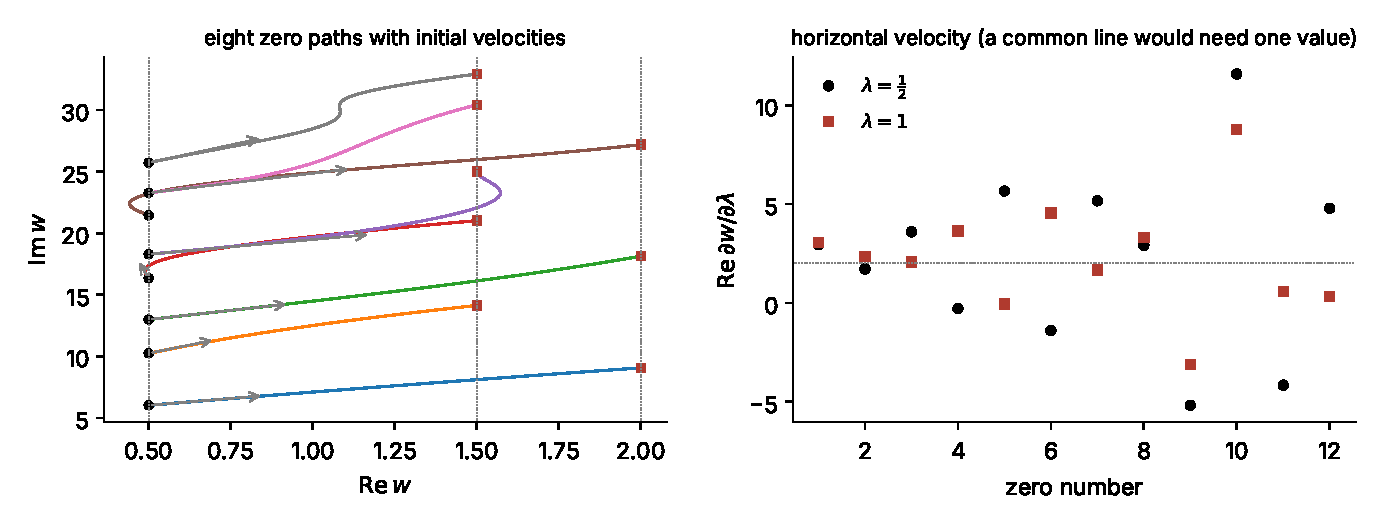
\includegraphics[width=\textwidth]{fig/v3/fig_mellin_velocity.pdf}
\caption{Left: paths of the first eight zeros from $\lambda=\frac12$ to $\lambda=1$, with arrows along the initial velocities. Right: real part of the velocity at the two ends for twelve zeros; a common line would need a single value.}
\label{ml:fig:velocity}
\end{figure}
A second run follows the first twelve zeros from $\lambda=\frac12$ to $\lambda=1$ with the velocity of Proposition~\ref{ml:prop:vel} as predictor and Newton's method with the exact derivative as corrector, and the results of the first run are reproduced (computed). All twelve paths end at $\lambda=1$ on known zeros. Eight end on the first eight zeros of $\zeta$, in order, at heights $14.1347$, $21.0220$, $25.0109$, $30.4249$, $32.9351$, $37.5862$, $40.9187$ and $43.3271$, and four on the first four zeros of $1-2^{2-w}$. Writing $P$ for a zero of $1-2^{2-w}$ and $z$ for a zero of $\zeta$, the pattern is $P,z,P,z,z,P,z,z,P,z,z,z$. At $\lambda=\frac34$ the twelve real parts range from $0.742$ to $1.486$. The argument principle gives a check that no zero is missed: at $\lambda=\frac34$ the winding number of $G_\lambda$ around the box $0.3\le\Re w\le3.2$, $5\le\Im w\le30.79$ is $8.000$ (to $10^{-14}$), and exactly eight tracked zeros lie in it, while the box $0.5\le\Im w\le5$ has winding number $0$ (computed, floating point).

\section{What the family shows}\label{ml:sec:meaning}
The statement the computation earns is the following.
\begin{proposition}[the shift of the lattice does not force a line; computed]\label{ml:prop:noline}
Let $\mathcal C$ be a condition on Thorin measures that every $\sum_{k\ge0}\delta_{2(k+\lambda)^2}$ with $\lambda\in[\frac12,1]$ satisfies. Then $\mathcal C$ does not imply that the zeros of the Mellin transform lie on one vertical line. In particular none of the following suffices: being an exponential series, having a P\'olya frequency density, having rates on a shifted quadratic lattice, or having a Laplace transform that is a ratio of Gamma functions.
\end{proposition}
Near $\lambda=\frac12$ this rests on Proposition~\ref{ml:prop:leave}, an explicit formula evaluated at twelve zeros. Away from the ends it rests on the tracked positions, supported by the argument principle count. All of it is floating point. The proposition must be read for what it says. At $\lambda=1$ alone the zeros of $\eta(w-1)$ lie on the two lines $\Re w=\frac32$ and $\Re w=2$, so a condition forcing one line for the whole zero set is excluded without any tracking. The content is for the family as a whole, and for the zeros that descend from $\beta$ and stay in the interior of the strip. Problem~\ref{kr:prob:mellin} asks for more: it asks about the zeros after the elementary factor is divided out, and for intermediate $\lambda$ there is no elementary factor, so the family does not test that form cleanly. It also does not exclude a Thorin condition that singles out the two ends. A condition such as closure of the atoms under multiplication up to a scale holds for $\{2n^2\}$ and for $\{(2n+1)^2/2\}$ and fails for the other shifted lattices. Problem~\ref{kr:prob:mellin} therefore stays open, and what is closed is the weaker claim that invariance under the shift of the lattice is enough.

What distinguishes $\lambda=\frac12$ and $\lambda=1$ is arithmetic. At the two ends $Z_{2\lambda}$ is the Dirichlet series of an $L$ function, or of one times a Dirichlet polynomial, and Hecke's correspondence \cite{Hecke36} turns the modular relation of the theta function into a functional equation. For other $\lambda$ the coefficients $(2\lambda)_k/k!$ are not periodic or polynomial of the right parity, and no inversion formula is known. When $2\lambda$ is an integer the function $Z_{2\lambda}$ is a finite combination of shifted $\beta$ or $\eta$ functions (Theorem~\ref{lv:thm:meixner}), which satisfy different functional equations piecewise. A functional equation does not put the zeros on a line by itself: the function of Davenport and Heilbronn \cite{DH36} has one and has zeros off the line. What the ends add is an Euler product.

Two things survive. The family is an explicit deformation through GGCs that carries the zeros of $\beta$ to those of $\zeta$, on which a proposed criterion for zeros on a line can be tested. And the reflection formula of Theorem~\ref{ml:thm:mellin} writes $D(-s)$ as a Mellin transform of $L$, a property shared by the whole family, which the experiment shows to be insufficient as well.

\section{Structure that holds for every $\lambda$}\label{ml:sec:structure}
Write $h_\lambda(t)=(2\cosh\frac t2)^{-2\lambda}$, so that $\Gamma(w)Z_{2\lambda}(w)=\int_0^\infty t^{w-1}h_\lambda(t)\,dt$ for $\Re w>0$. That $Z_{2\lambda}$ is entire and vanishes at the negative odd integers is part of Theorem~\ref{lv:thm:meixner}. The values at the nonpositive integers are not stated there.
\begin{theorem}\label{ml:thm:trivial}
For every $\lambda>0$ and $n=0,1,2,\dots$, $Z_{2\lambda}(-n)=(-1)^nh_\lambda^{(n)}(0)$. In particular $Z_{2\lambda}(0)=4^{-\lambda}$ and $Z_{2\lambda}(-2)=-\frac\lambda2\,4^{-\lambda}$.
\end{theorem}
\begin{proof}
$h_\lambda$ is smooth and even at $0$ and decays exponentially. Split the integral at $t=1$ and expand $h_\lambda(t)=\sum_ja_{2j}t^{2j}$ on $(0,1)$: the Mellin integral continues to a meromorphic function whose only poles are simple, at $w=-2j$, with residue $a_{2j}$. Division by $\Gamma(w)$, which has residue $(-1)^n/n!$ at $-n$, removes the poles and gives $Z_{2\lambda}(-2j)=(2j)!\,a_{2j}$ and $Z_{2\lambda}(-(2j+1))=0$. The two values follow from $h_\lambda(t)=4^{-\lambda}(1-\frac{\lambda}{4}t^2+\dots)$.
\end{proof}
At $\lambda=\frac12$ these are the trivial zeros of $\beta$ and at $\lambda=1$ those of $\zeta(w-1)$. They do not move with $\lambda$: they come from the evenness of the hyperbolic secant, not from arithmetic. At $\lambda=\frac34$ the series gives $Z_{3/2}(0)=0.3535534=4^{-3/4}$, $Z_{3/2}(-2)=-0.1325825$, and $Z_{3/2}$ at $-1$, $-3$, $-5$ and $-7$ is of size $10^{-30}$, the working precision (computed).
\begin{theorem}[zero free half plane]\label{ml:thm:right}
Let $\sigma_0(\lambda)>2\lambda$ be the root of
\[\sum_{k\ge1}\frac{(2\lambda)_k}{k!}\Big(\frac{\lambda}{k+\lambda}\Big)^{\sigma}=1.\]
Then $Z_{2\lambda}(w)\ne0$ for $\Re w>\sigma_0(\lambda)$.
\end{theorem}
\begin{proof}
The terms are positive and the sum is finite for $\sigma>2\lambda$ and decreases to $0$ as $\sigma\to\infty$, so the root exists. For $\Re w>\sigma_0$ the first term $\lambda^{-w}$ of the series exceeds in modulus the sum of the others, which is at most $\lambda^{-\Re w}\sum_{k\ge1}\frac{(2\lambda)_k}{k!}(\lambda/(k+\lambda))^{\Re w}<\lambda^{-\Re w}$.
\end{proof}
The values are $\sigma_0=1.37$, $2.04$ and $2.73$ at $\lambda=\frac12$, $\frac34$ and $1$ (computed; at $\lambda=\frac12$ the equation is $(1-2^{-\sigma})\zeta(\sigma)=2$). The first twelve zeros that we follow have real parts at most $0.5$, $1.49$ and $2$ at those levels.

Two statements about the left half plane and the zero count are heuristic, not proved. We state them because the main term is correct at both ends and the computed zeros follow it.
\begin{remark}[left half plane; heuristic]\label{ml:rem:left}
As $\Re w\to-\infty$,
\[
Z_{2\lambda}(w)\approx\frac{2}{\Gamma(2\lambda)}\,\pi^{w-2\lambda}\,\Gamma(2\lambda-w)\,\cos\frac{\pi w}{2}\,\big(1+O(|w|^{-2})\big).
\]
Write $Z_{2\lambda}$ as a Hankel loop integral of $(-t)^{w-1}h_\lambda(t)$ and move the loop outwards for $\Re w<0$. The singularities of $h_\lambda$ are branch points at $t=\pm i\pi(2m+1)$, where $2\cosh\frac t2$ vanishes to first order, and the pair nearest the origin dominates: it contributes $\Gamma(2\lambda-w)/\Gamma(2\lambda)$ times $(\pm i\pi)^{w-2\lambda}$, with phases that combine to the cosine, and the next pair is smaller by $3^{\Re w}$. Near $t=\pm i\pi$ the singularity is $(iu)^{-2\lambda}(1-\frac\lambda{12}u^2+\dots)$ in the local variable $u$, which gives the relative order $|w|^{-2}$. The error bound is not written out. Three checks support the formula. The cosine reproduces the trivial zeros of Theorem~\ref{ml:thm:trivial}. At $\lambda=\frac12$ and $\lambda=1$ it is the functional equation of $\beta$ and of $\eta$, with the factors $\beta(1-w)$ and $(1-2^{w-2})\zeta(2-w)$ in place of $1$. And at $\lambda=\frac34$ the ratio of the two sides is $1.0034-0.0201i$ at $w=-2.5+3i$, $0.9985-0.0013i$ at $w=-8.5+3i$ and $0.9996-0.0003i$ at $w=-16.5+5i$ (computed).
\end{remark}
So $Z_{2\lambda}$ has half of a functional equation for every $\lambda$: the Gamma factor and the trivial zeros are always there. At the two ends the remaining factor is again a Dirichlet series of the same kind.

Let $N_\lambda(T)$ be the number of zeros of $Z_{2\lambda}$ with $0<\Im w<T$.
\begin{remark}[counting law; heuristic]\label{ml:rem:count}
Define $S_\lambda(T)$ by
\[
N_\lambda(T)=\frac{T}{2\pi}\log\frac{T}{\pi e\lambda}+\frac\lambda2-\frac18+S_\lambda(T).
\]
The content is the claim $S_\lambda(T)=O(\log T)$ uniformly for $\lambda\in[\frac12,1]$, which is not proved. The main term comes from the argument principle on the rectangle with corners $-A+i\varepsilon$, $\sigma_0+i\varepsilon$, $\sigma_0+iT$, $-A+iT$, as in the classical count \cite[Chapters 15 and 16]{Davenport}. On the right side $Z_{2\lambda}$ is $\lambda^{-w}$ times a factor with positive real part (Theorem~\ref{ml:thm:right}), so the argument there is $-T\log\lambda+O(1)$. On the left side the argument is given by Remark~\ref{ml:rem:left}, and Stirling's formula for $\arg\Gamma(2\lambda-w)$ gives $-T\log T+T+(2\lambda-\frac12)\frac\pi2$, to which $\pi^w$ adds $T\log\pi$. The difference divided by $2\pi$ is the main term. The remaining pieces are the variation of the argument along the top edge, divided by $2\pi$ (not $\pi$, since $Z_{2\lambda}$ has no functional equation to halve it), and the bounded contribution of the right edge; both are in $S_\lambda$.
\end{remark}
At $\lambda=\frac12$ the main term is the classical formula $\frac{T}{2\pi}\log\frac{2T}{\pi e}+\frac18$ for the character modulo $4$. At $\lambda=1$ it is the sum of $\frac{T}{2\pi}\log\frac{T}{2\pi e}+\frac78$ for $\zeta$ and $\frac{T\log2}{2\pi}-\frac12$ for the zeros of $1-2^{2-w}$. The constant $\frac\lambda2-\frac18$ was first seen in the data and then traced to Stirling's formula. Computed against the tracked zeros of the next section, the count differs from the main term by less than $0.5$ in absolute value at each of twenty pairs $(\lambda,T)$, with $\lambda\in\{0.5,0.6,0.75,1\}$ and $T\in\{20,40,60,80,100\}$ (computed); at $\lambda=1$ the tracked count equals the exact count of zeros of $\eta(w-1)$, namely $3$, $19$ and $40$ at $T=20,60,100$. Over the whole range $20\le T\le100$ the residual shown in Figure~\ref{ml:fig:pairing} stays below $1$ in absolute value.% UNVERIFIED: the residual below 1 over 20 <= T <= 100 in steps of 1/2 and the earlier table of its mean (the verification tested twenty points only)

Three consequences follow from the main term, each heuristic.
\begin{itemize}
\item Flux. As $\lambda$ goes from $\frac12$ to $1$ the number of zeros below height $T$ falls by $N_{1/2}(T)-N_1(T)=\frac{T\log2}{2\pi}-\frac14$, the number of zeros of $1-2^{2-w}$ below $T$ up to a bounded term.
\item Speed. If the $n$th zero keeps its rank, its height $T(\lambda)$ solves $N_\lambda(T)=n$, and implicit differentiation of the main term gives $\dfrac{dT}{d\lambda}=\dfrac{T/\lambda-\pi}{\log\frac{T}{\pi\lambda}}$, which is $\dfrac{T}{\lambda\log\frac{T}{\pi\lambda}}$ up to the term $\pi$. At $\lambda=\frac12$ the ratio of the true vertical velocity (Proposition~\ref{ml:prop:vel}) to the approximate prediction averages $0.975$ over zeros $11$ to $54$, and the dropped term $\pi$ accounts for most of the gap.% UNVERIFIED: the average 0.975
\item Proportion. Granted the pairing conjecture below, the share of zeros of $\beta$ below $T$ that end on zeros of $1-2^{2-w}$ is about $\log2/\log\frac{2T}{\pi e}$ and tends to zero. Among the first $54$ it is $13$ of $54$.
\end{itemize}

\section{The pairing of the first 54 zeros, computed}\label{ml:sec:pairing}
We found the $54$ zeros of $\beta$ with height below $106$ by sign changes of the completed function on the critical line. The smooth count at $106$ is $54.3$ with the constant $\frac18$. All $54$ lie on $\Re w=\frac12$ to $10^{-40}$ (computed, ball arithmetic at four hundred bits). We followed each to $\lambda=1$ by a predictor and corrector scheme: the velocity formula predicts, Newton's method corrects, and the step in $\lambda$ is halved until the correction is small. The step matters. Zeros $37$, $38$, $52$ and $53$ turn sharply, with $\Re w$ moving by $0.5$ to $0.7$ within $0.05$ in $\lambda$ (zero $38$ has $\Re w=1.161$ at $\lambda=0.6$ and $0.43$ at $0.65$), and a fixed step of $0.005$ jumps to a wrong root there. An independent run with adaptive steps, the smallest $7.8\times10^{-5}$, reproduces everything below.
\begin{proposition}[pairing of the first $54$ zeros; computed]\label{ml:prop:pair}
Continuation in $\lambda$ from $\frac12$ to $1$ maps the first $54$ zeros of $\beta$ one to one onto the first $54$ zeros of $\eta(w-1)$ in order of height: $41$ zeros of $\zeta$, shifted to $\Re w=\frac32$, and $13$ zeros of $1-2^{2-w}$ on $\Re w=2$. The end points agree with the known zeros to $2\times10^{-14}$. The first $24$ zeros keep their rank, and the map on ranks is the permutation
\[(25\ 26)\,(29\ 30)\,(38\ 39\ 40)\,(47\ 48)\,(53\ 54).\]
No tracked zero leaves the half plane $\Re w>0.11$; the smallest real part is $0.1145$, at zero $30$ and $\lambda=0.535$.
\end{proposition}
The status is computed in floating point, not certified: Newton corrections of size $0.05$ at the first step, small against the closest approach of the paths, give no certificate against a jump between paths. Heights are not monotone along the paths: $225$ adjacent order inversions occur over the $101$ grid values of $\lambda$, so zeros cross in height, and the permutation records the net effect. The note further states that no two zeros collide, the closest approach being $0.131$ between zeros $38$ and $39$ at $\lambda=0.625$, that every zero stays in $\Re w<2.26$, that all but eleven of the $54$ zeros keep their rank for every $\lambda$, and that the twelve paths involved in rank changes move by less than $3\times10^{-10}$ under a refinement of the steps (computed in the note, not rechecked).% UNVERIFIED: closest approach 0.131 at lambda 0.625, Re w < 2.26, all but eleven keep rank, refinement 3e-10

\begin{figure}[t]
\centering
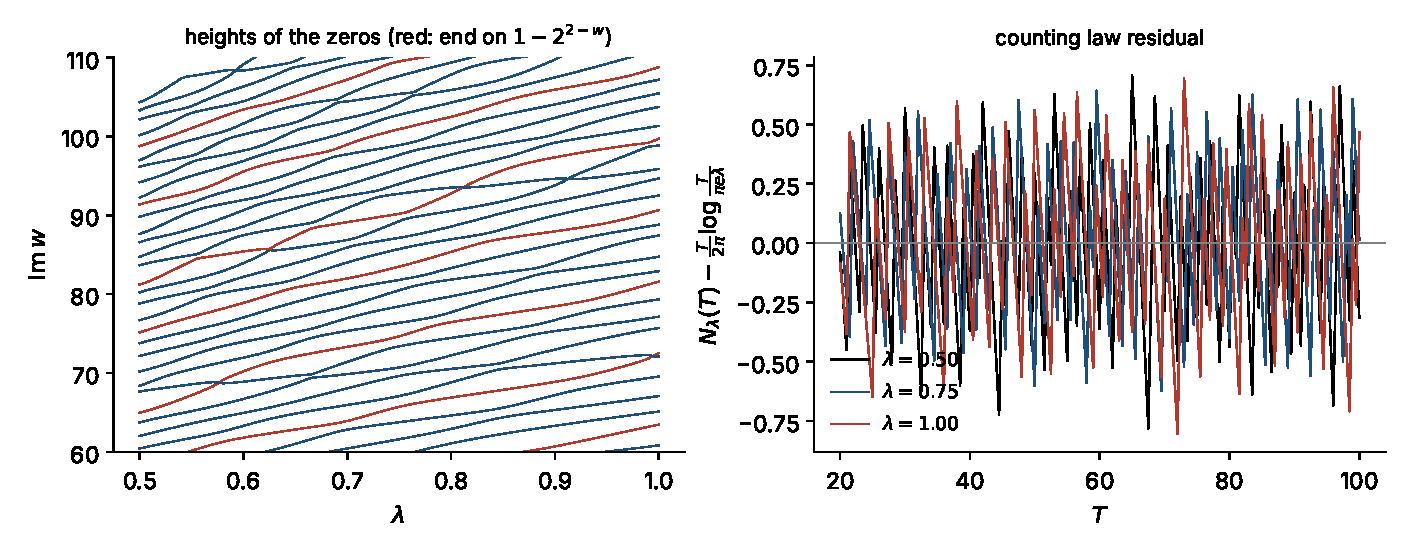
\includegraphics[width=\textwidth]{fig/v3/fig_pairing.pdf}
\caption{Left: heights of the zeros against $\lambda$, in the window where ranks change; paths that end on zeros of $1-2^{2-w}$ are red. Right: the residual $S_\lambda(T)$ of the counting law at three levels.}
\label{ml:fig:pairing}
\end{figure}
The table lists the eleven zeros whose rank changes.
\begin{center}
\small
\begin{tabular}{clll}
\toprule
zero of $\beta$ & height & ends at & rank\\
\midrule
25 & $58.12$ & $2+72.518\,i$, zero of $1-2^{2-w}$ & 26\\
26 & $60.42$ & $\frac32+72.067\,i$, $\gamma_{18}$ & 25\\
29 & $64.98$ & $2+81.582\,i$, zero of $1-2^{2-w}$ & 30\\
30 & $67.64$ & $\frac32+79.337\,i$, $\gamma_{21}$ & 29\\
38 & $80.21$ & $\frac32+98.831\,i$, $\gamma_{29}$ & 39\\
39 & $81.21$ & $2+99.712\,i$, zero of $1-2^{2-w}$ & 40\\
40 & $83.67$ & $\frac32+95.871\,i$, $\gamma_{28}$ & 38\\
47 & $94.17$ & $\frac32+114.320\,i$, $\gamma_{36}$ & 48\\
48 & $96.14$ & $\frac32+111.875\,i$, $\gamma_{35}$ & 47\\
53 & $103.29$ & $\frac32+124.257\,i$, $\gamma_{41}$ & 54\\
54 & $104.33$ & $\frac32+122.947\,i$, $\gamma_{40}$ & 53\\
\bottomrule
\end{tabular}
\end{center}
Here $\gamma_n$ is the ordinate of the $n$th zero of $\zeta$. Four remarks.
\begin{itemize}
\item Pairing by rank is false. The first failure, at zeros $25$ and $26$, happens at $\lambda=0.995$: the two targets are $0.45$ apart in height but on different lines, and the paths cross in height without meeting. This kind of exchange is harmless.% UNVERIFIED: the value lambda=0.995
\item The exchanges $(47\ 48)$ and $(53\ 54)$ have two zeros of $\zeta$ as targets, and the heights cross early, at $\lambda=0.915$ and $\lambda=0.595$, while the two zeros are at different real parts. In the cycle $(38\ 39\ 40)$ the zeros $38$ and $40$ end at $\gamma_{29}$ and $\gamma_{28}$, so the order of two targets is reversed there too. Three of the five cycles therefore reorder zeros of $\zeta$, and even the map from the zeros of $\beta$ to the zeros of $\zeta$ alone does not preserve order.% UNVERIFIED: the lambda values 0.915 and 0.595
\item The rank changes are local. No zero moves by more than two places, in agreement with the residual of the counting law staying below $1$.
\item The horizontal motion is not monotone on every path. The note reports a horizontal velocity at $\lambda=\frac12$ ranging from $-34.0$ to $34.0$ over the $54$ zeros, against $-5.2$ to $11.6$ over the first twelve, and takes this as support for the guess that it is unbounded in both directions. The symmetry to three digits should be rechecked before anyone relies on it.% UNVERIFIED: the range -34.0 to 34.0
\end{itemize}

\section{What is proved, and what is open}\label{ml:sec:open}
Proved, for all $\lambda>0$: Theorems~\ref{ml:thm:mellin}, \ref{ml:thm:family}, \ref{ml:thm:trivial} and \ref{ml:thm:right}, and Proposition~\ref{ml:prop:vel}. Computed in floating point: Propositions~\ref{ml:prop:leave}, \ref{ml:prop:noline} and \ref{ml:prop:pair}. Heuristic: Remarks~\ref{ml:rem:left} and \ref{ml:rem:count}. Nothing in this chapter is a step towards RH. The pairing is a statement about how the zeros of two $L$ functions are joined through functions that are not $L$ functions, and the absence of order in the join is one more sign that the line is not carried by the family.
\ifdefined\conjecture\else\theoremstyle{sc}\newtheorem{conjecture}[theorem]{Conjecture}\theoremstyle{scr}\fi
\begin{conjecture}[pairing]\label{ml:conj:pairing}
For every $\lambda\in[\frac12,1]$ the zeros of $Z_{2\lambda}$ in $\Im w>0$ are simple. Continuation in $\lambda$ is a one to one map from the zeros of $\beta$ onto the zeros of $\eta(w-1)$ in the upper half plane, and it moves the rank of a zero of height $T$ by $O(\log T)$ at most.
\end{conjecture}
\begin{problem}\label{ml:prob:count}
Complete the heuristic of Remark~\ref{ml:rem:left} with an explicit error term and deduce $S_\lambda(T)=O(\log T)$ uniformly for $\lambda\in[\frac12,1]$. The polynomial bound for $Z_t$ on vertical lines is in the proof of Corollary~\ref{lv:cor:meixner}, and with Phragm\'en and Lindel\"of on a strip the argument of Backlund gives the bound on $S_\lambda$ once the uniform error term is available; that term is a routine Hankel and Darboux estimate at the singularities $t=\pm i\pi$. With simplicity of the zeros this gives the conjecture.
\end{problem}
\begin{problem}\label{ml:prob:simple}
Show that $Z_{2\lambda}$ and $\partial_wZ_{2\lambda}$ have no common zero for real $\lambda$. Double zeros are isolated points of complex codimension two in the pair $(\lambda,w)$ for complex $\lambda$, so for real $\lambda$ they are not expected, but the approach of the paths to within $0.131$ (the value of the note) shows that they are near.
\end{problem}
\begin{problem}\label{ml:prob:perm}
Predict the permutation. Is an exchange of ranks decided by the two targets at $\lambda=1$, or by the near double zeros at complex $\lambda$ around which the paths braid? Is the displacement of rank bounded? In $54$ zeros it is at most $2$.
\end{problem}
\begin{problem}\label{ml:prob:vel}
Make Proposition~\ref{ml:prop:leave} certified with interval arithmetic, and prove that $\Re\,\partial w/\partial\lambda$ is unbounded in both directions along the zeros of $\beta$, as the table suggests. Express the velocity at $\lambda=\frac12$ through $\beta$ itself: the numerator of Proposition~\ref{ml:prop:vel} is the Mellin transform of $\log(2\cosh\frac t2)\operatorname{sech}\frac t2$, which gives a term in $\beta(w+1)$ and a double sum $\sum_{k,m}(-1)^{k+m-1}m^{-1}(k+m+\frac12)^{-w}$, an additive and not a Dirichlet convolution.
\end{problem}
\begin{problem}\label{ml:prob:which}
Which zeros of $\beta$ go to zeros of $\zeta$ and which to zeros of $1-2^{2-w}$? Among the first twelve the pattern is $P,z,P,z,z,P,z,z,P,z,z,z$. The counting functions force the proportion (Remark~\ref{ml:rem:count}), not the pattern, and the pairing computation of Section~\ref{ml:sec:pairing} shows that it is not decided by rank alone beyond the first $24$ zeros.
\end{problem}
